\section{Hour Estimation}

	This section describes what hour estimation is, how to perform it and how we did 
	include it in our project. The actual estimated hours is not done in this section, 
	but is documented in each sprint section.

	{\bf What is hour estimation?} Hour estimation is a part of project to be able to ensure the 
	deadline and resources needed to complete a project in time.
	Hour estimation can be done in many different ways, but it often depends on the methodology
	used in the project. 
	In a waterfall project, it is often normal to do all the estimation in the start of a project.
	When a project is doing agile methods like scrum, it is often normal to do the estimation part
	in each sprint. 

	{\bf Why perform hour estimation?} In software projects, the projects normally starts with
	a planning phase and a hour estimation. This is estimation is done for many reasons:
		\begin{itemize}
			\item Calculate the cost for delivering a project.
			\item Calculation resouces for a project (e.g how many people do the team 
			need for this project?).
			\item How many features can the team implement during a phase/sprint?
			\item Are the project in time (the estimated hours in the backlog)?
			\item How big is this project in terms of hours?
		\end{itemize}
	There are many good reasons for doing a estimation, but the reasons are often dependent
	of the methodology used and the purpose of the project. 

	If a project have not done any estimations, there is many risk factors that can apper. 
	Here are some risks that can appear when not doing hour estimation:
	\begin{itemize}
		\item If a company win a project and promises the customer to deliver at a 
		specified date without estimating hours for the project, there is a big risk 
		that the project will fail.
		\item If a project have not estimated the hours, there is a possibility that 
		there is not allocated enough resources for the project, and the project could 
		be risking not to be delivered at the planned date.  
	\end{itemize}

	{\bf How we performed hour estimation} This project have like many other projects a deadline
	as well as a specified number of resources. In many projects it is normal to set the wanted 
	delivery and then estimate the number of resources needed to deliver the project.
	In this project we started with a number of resources (4 students) and then planned the 
	delivery based on the workload of the course (ca 24 hours/persons/week). The actual 
	hour estimation is done in the start of every sprint. The reason for doing this is because of 
	the chosen methodology scrum.

	\begin{figure}[H]
		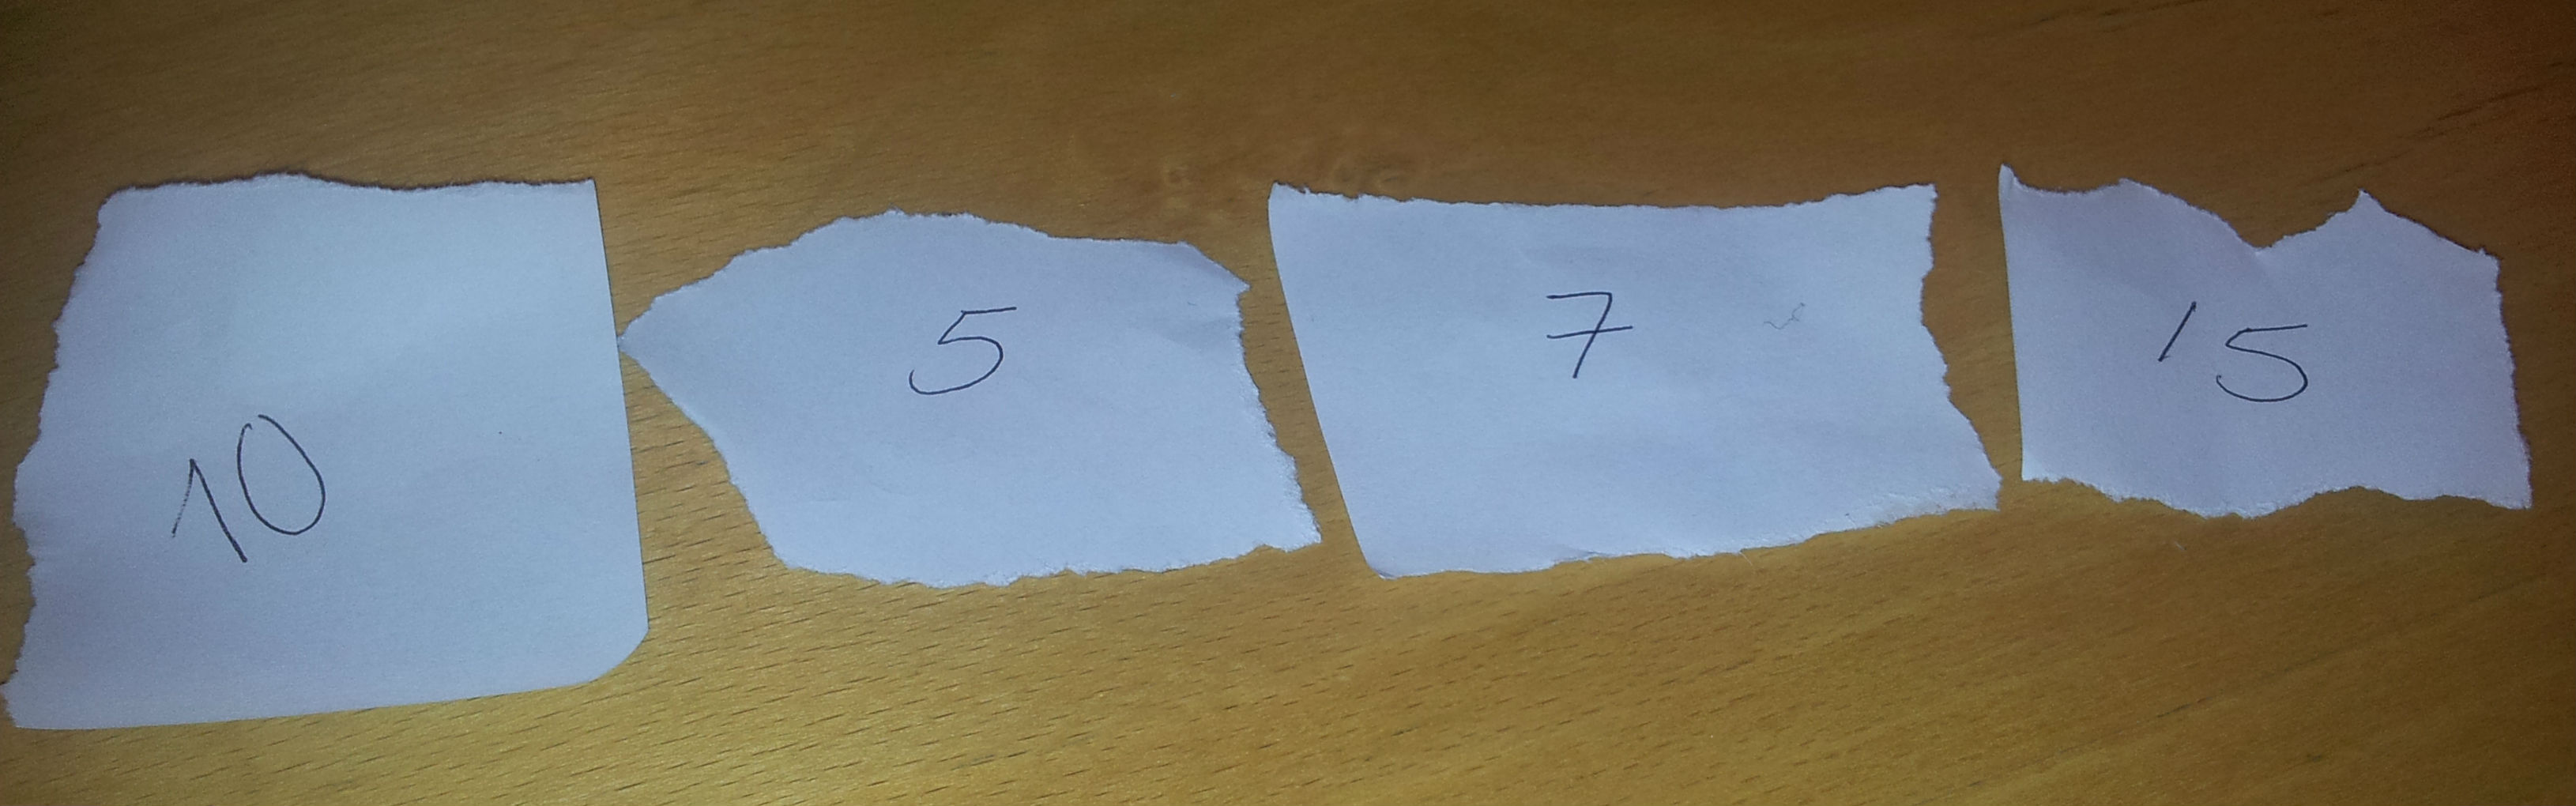
\includegraphics[width=1.0\textwidth]{pictures/estimation.jpg}
	\end{figure}

	In the start of every sprint, the group sat down for a hour estimation for the sprint.
	Before the hour estimation, it the sprint backlog was planned. For every functional requirement
	in the sprint backlog, every person in the scrum team wrote down a guessed hour estimate
	for the functional requirement. After showing all the estimates, we chose the avarage of
	the estimates.The reason for doing the estimation in this way is because the group 
	are quite unexperienced with hour estimation. When doing it in this way, some team 
	members will overestimate and some will underestimate and the result will often be a estimate that is close to the actual effort. 
